\section{Bilan de liaison}

\href{https://youtu.be/qFMQgfgPAvg}{Introduction au budget de liaison par satellite – Partie 11.}

\href{https://youtu.be/FTHt-c8hWKw}{Introduction au budget de liaison par satellite – Partie 12.}

L'équation du bilan de liaison est la relation fondamentale qui guide la conception de l'architecture des communications. Elle relie les exigences (débit de données, taux d'erreur binaire) aux principaux paramètres de conception du sous-système de communication du satellite et du segment sol. Cette équation peut être modifiée pour assurer la fermeture du bilan de liaison.

Les considérations de conception incluent :

\begin{itemize}
    \item Exigences sur la taille des antennes
    \item Niveaux de puissance de transmission
    \item Bruit acceptable au récepteur
    \item Choix de la fréquence de transmission
\end{itemize}

L'équation du bilan de liaison est :

\begin{equation}
    \frac{E_b}{N_0} = \frac{P_t G_t G_r L_a L_l \lambda^2}{(4\pi R)^2 k T R_b} > \frac{E_b}{N_{0,min}}
\end{equation}

où :
\begin{itemize}
    \item $P_t$ : Puissance de transmission (Watts)
    \item $L_l$ : Pertes entre l'émetteur et l'antenne (sans unité, Watts/Watts)
    \item $G_t$ : Gain de l'antenne émettrice (sans unité, Watts/Watts)
    \item $L_s$ : Pertes dans l'espace libre (sans unité, Watts/Watts)
    \item $L_a$ : Pertes sur le chemin de transmission (sans unité, Watts/Watts)
    \item $G_r$ : Gain de l'antenne réceptrice (sans unité, Watts/Watts)
    \item $k$ : Constante de Boltzmann (Joules/Kelvin)
    \item $T_s$ : Température de bruit du système (Kelvin)
\end{itemize}

Expressions intermédiaires :

\begin{itemize}
    \item Densité de flux de puissance à une distance $R$ :
    \begin{equation}
        W_t = \frac{P_t G_t}{(4\pi R)^2}
    \end{equation}
    
    \item Effet des pertes atmosphériques et des circuits :
    \begin{equation}
        W_r = W_t L_a L_l
    \end{equation}
    
    \item Puissance reçue :
    \begin{equation}
        P_r = W_r \cdot A_{eff} = W_r \cdot \frac{\lambda^2}{4\pi} G_r
    \end{equation}
    
    \item Énergie par bit :
    \begin{equation}
        E_b = \frac{P_r}{R_b}
    \end{equation}
    
    \item Bruit :
    \begin{equation}
        N_0 = kT
    \end{equation}
\end{itemize}

En combinant toutes ces expressions, l'équation finale du bilan de liaison est :

\begin{equation}
    \frac{E_b}{N_0} = \frac{P_t G_t G_r L_a L_l \lambda^2}{(4\pi R)^2 k T R_b} > \frac{E_b}{N_{0,min}}
\end{equation}

En forme logarithmique, en utilisant les définitions :

\begin{itemize}
    \item Puissance isotrope rayonnée équivalente (EIRP) :
    \begin{equation}
        EIRP \equiv P_t G_t
    \end{equation}
    
    \item Pertes en espace libre :
    \begin{equation}
        L_s \equiv \frac{\lambda^2}{(4\pi R)^2}
    \end{equation}
    
    \item Rapport Gain sur Température de bruit :
    \begin{equation}
        \frac{G_r}{T}
    \end{equation}
\end{itemize}

Tous les paramètres en dB :

\begin{equation}
    \frac{E_b}{N_0} (\text{dB}) = EIRP (\text{dBW}) + L_S (\text{dB}) + L_a (\text{dB}) + L_l (\text{dB}) + \frac{G_r}{T} \left(\frac{\text{dB}}{K}\right) - 10 \log k - 10 \log R_b
\end{equation}

Le gain d'antenne est un paramètre clé en électromagnétisme, combinant la directivité de l'antenne et son efficacité électrique.

\begin{figure}[H] % H force l'affichage ici
    \centering
    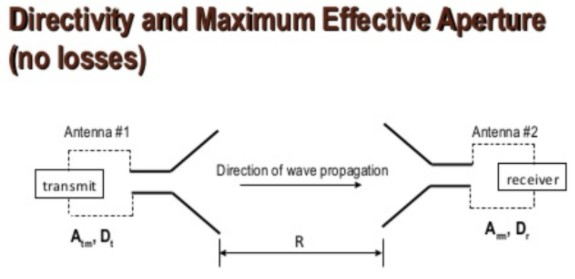
\includegraphics[width=0.8\textwidth]{figures/6-51.jpg}
    
    \caption{Directivity and maximum effective aperture diagram. Image by AJAL A.}
    \label{fig:communication2}
\end{figure}


Quelle que soit la situation, l'expression générale du gain d'antenne est :

\begin{equation}
    G = \eta \frac{4 \pi}{\lambda^2} A = \frac{\eta 4 \pi}{\lambda^2} D_t D_r
\end{equation}

où :

\begin{itemize}
    \item $\eta$ est le rendement de l'antenne, défini par le rapport entre la puissance sortante et la puissance entrante : $\frac{P_o}{P_{in}}$
    \item $4 \pi$ représente le nombre de stéradians dans une sphère, utilisé pour calculer le rayonnement moyen indépendamment de la directivité.
    \item $\lambda$ est la longueur d'onde.
    \item $A$ est la surface d'ouverture efficace.
    \item $D$ est la directivité associée à l’émetteur ou au récepteur.
\end{itemize}

La résolution angulaire obtenue par une ouverture est donnée par :

\begin{equation}
    \theta = \alpha \frac{\lambda}{D}
\end{equation}

où $\alpha = 1.22$ pour une ouverture circulaire et $\alpha = 1$ pour une ouverture rectangulaire.

\begin{figure}[H] % H force l'affichage ici
    \centering
    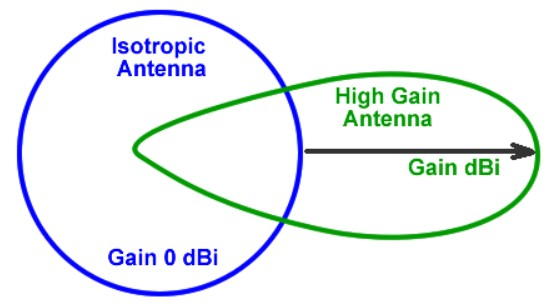
\includegraphics[width=0.8\textwidth]{figures/6-52.jpg}
    
    \caption{Antenna gain pattern. Image by Electronics 360.}
    \label{fig:communication2}
\end{figure}


Les gains pour différentes formes d'antennes sont :

\begin{itemize}
    \item Antenne omnidirectionnelle : $G = 1$ (0 dB)
    \item Antenne parabolique d’ouverture $D$ : 
    \begin{equation}
        G = \eta \left(\frac{\pi D}{\lambda}\right)^2
    \end{equation}
    \begin{itemize}
        \item Valeurs typiques : $\eta = 0.55 - 0.6$
    \end{itemize}
    \item Antenne hélicoïdale :
    \begin{equation}
        G(dB) \approx 10.25 + 1.22 \frac{L}{\lambda} - 0.0726 \left(\frac{L}{\lambda}\right)^2
    \end{equation}
    où $L$ est la longueur de l’antenne.
    
    \item Ce gain est obtenu lorsque le rayon $R$ satisfait la condition :
    \begin{equation}
        \frac{R}{\lambda} = 0.2025 - 0.0079 \frac{L}{\lambda} + 0.000515 \left(\frac{L}{\lambda}\right)^2
    \end{equation}
\end{itemize}

\begin{figure}[H] % H force l'affichage ici
    \centering
    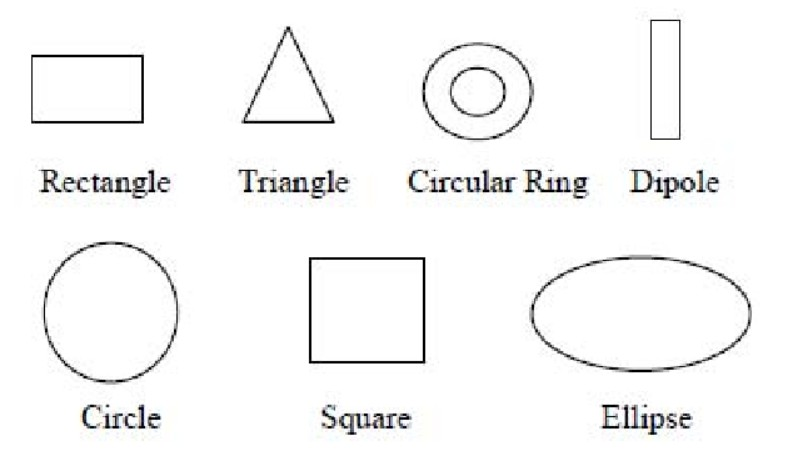
\includegraphics[width=0.8\textwidth]{figures/6-53.jpg}
    
    \caption{Various shapes of the patch antenna. Kiruthika, R., and T. Shanmuganantham. “Comparison of different shapes in microstrip patch antenna for X-band applications.” 2016 International Conference on Emerging Technological Trends (ICETT). IEEE, 2016.}
    \label{fig:communication2}
\end{figure}

\textbf{Puissance isotrope rayonnée équivalente}

\begin{figure}[H] % H force l'affichage ici
    \centering
    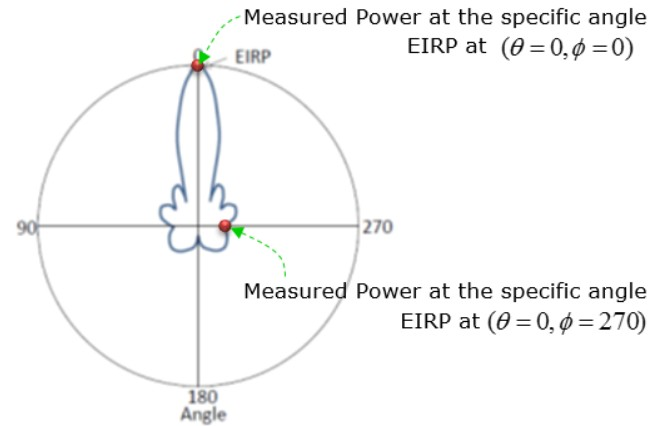
\includegraphics[width=0.8\textwidth]{figures/6-54.jpg}
    
    \caption{EIRP is a measurement showing performance at a specific point only (i.e, the measurement at a specific angle (Phi, Theta). Image by Share Tech Note}
    \label{fig:communication2}
\end{figure}


La Puissance Isotrope Rayonnée Équivalente (EIRP) est le principal paramètre de conception du côté de l’émetteur. L’EIRP est le produit de la puissance transmise et du gain de l’antenne émettrice. 

\textit{« La puissance isotrope rayonnée équivalente est la puissance hypothétique qui devrait être rayonnée par une antenne isotrope pour donner la même intensité de signal (équivalente) que l'antenne réelle dans la direction du faisceau le plus puissant de l'antenne »} [Wikipedia]. 

Cela signifie qu’il existe un compromis entre la taille de l’antenne et la puissance transmise. On peut compenser une petite antenne en transmettant plus de puissance, et inversement. Le choix de ce compromis dépend du coût ainsi que d’autres critères et contraintes (par exemple, des contraintes de volume). Formellement :

\begin{equation}
    EIRP = P_T - L_C + G_a
\end{equation}

où :

\begin{itemize}
    \item $P_T$ est la puissance de sortie de l’émetteur (dBm),
    \item $L_C$ est la perte dans les câbles (dB),
    \item $G_a$ est le gain de l’antenne émettrice (dB).
\end{itemize}

\begin{figure}[H] % H force l'affichage ici
    \centering
    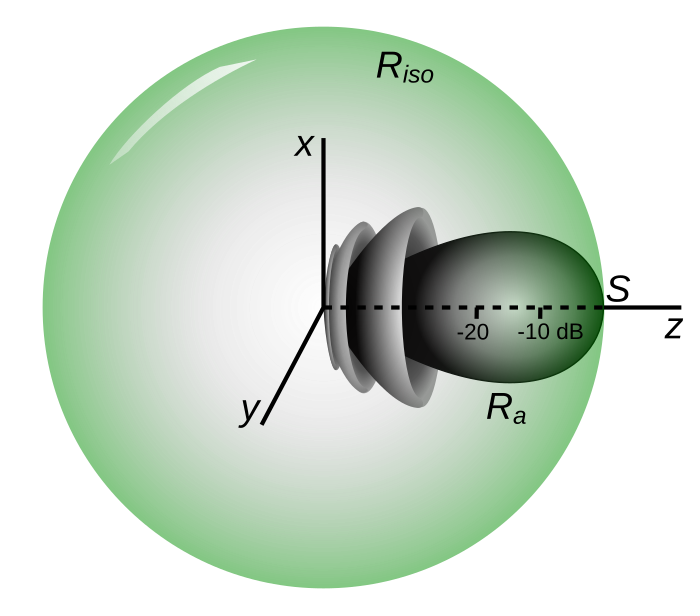
\includegraphics[width=0.8\textwidth]{figures/6-55.png}
    
    \caption{Illustration of the definition of equivalent isotropically radiated power (EIRP). The axes have units of signal strength in decibels. $R_a$ is the radiation pattern of a given transmitter driving a directional antenna. It radiates a far-field signal strength of S in its direction of maximum radiation (main lobe) along the z-axis. The green sphere $R_{iso}$ is the radiation pattern of an ideal isotropic antenna that radiates the same maximum signal strength as the directive antenna does. The transmitter power that would have to be applied to the isotropic antenna to radiate this much power is the EIRP. Image by Chet Vorno.}
    \label{fig:communication2}
\end{figure}

\textbf{Pertes en espace libre}

La perte de trajet en espace libre est l'atténuation de l'énergie radio entre les points d'alimentation de deux antennes, résultant de la combinaison de la zone de capture de l'antenne réceptrice et du trajet en ligne de vue sans obstacle à travers l'espace libre (généralement l'air) \cite{wikipedia}.

Formellement, la perte en espace libre est donnée par :
\begin{equation}
    L_s \equiv \frac{\lambda^2}{(4\pi R)^2}
\end{equation}

où \( R \) est la distance entre les antennes.  

La perte de trajet en espace libre est le facteur de perte dans cette équation qui est dû à la distance et à la longueur d'onde, ou en d'autres termes, le rapport entre la puissance transmise et la puissance reçue en supposant que les antennes sont isotropes et n'ont aucune directivité \cite{wikipedia}.

\begin{figure}[H] % H force l'affichage ici
    \centering
    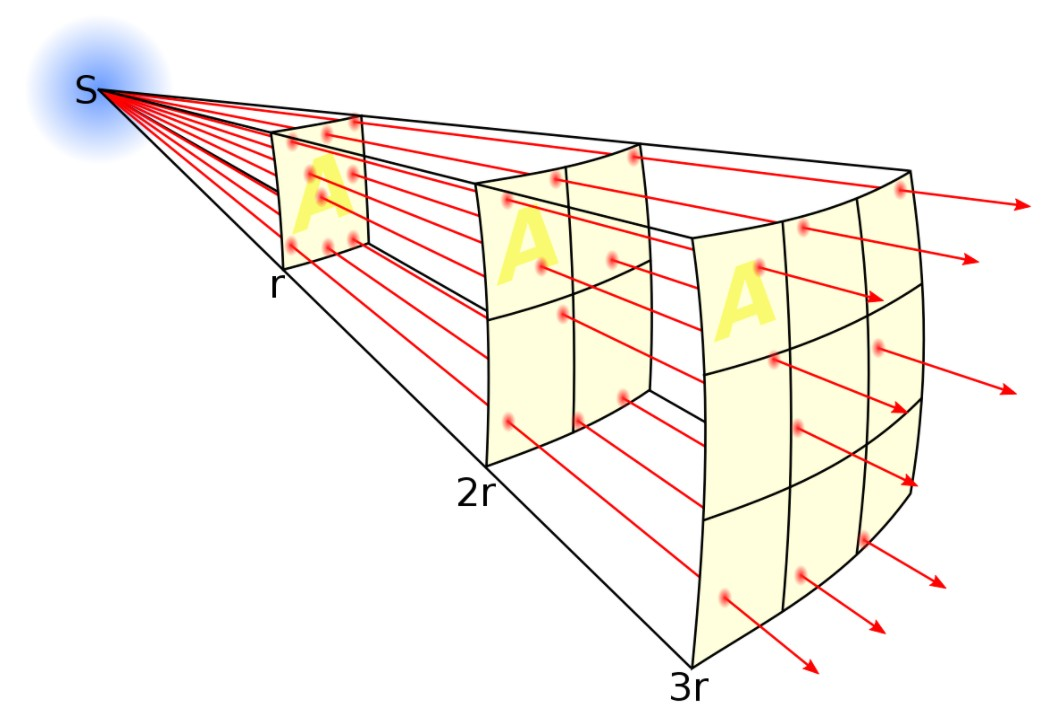
\includegraphics[width=0.8\textwidth]{figures/6-56.jpg}
    
    \caption{In free space, the intensity of electromagnetic radiation decreases with distance by the inverse square law, because the same amount of power spreads over an area proportional to the square of the distance from the source. CC BY-SA 3.0. Image by Borb.}
    \label{fig:communication2}
\end{figure}

\begin{itemize}
    \item \textbf{Pertes en espace libre}
    
    La perte en espace libre augmente avec la distance entre les antennes et diminue avec la longueur d'onde des ondes radio en raison de ces facteurs.

    \item \textbf{Intensité (\(I\))} 
    
    La densité de puissance des ondes radio diminue avec le carré de la distance par rapport à l'antenne émettrice, en raison de la dispersion de l'énergie électromagnétique dans l'espace selon la loi de l'inverse du carré.

    \item \textbf{Surface de capture de l'antenne (\(A_{eff}\))} 
    
    La quantité de puissance captée par l'antenne réceptrice à partir du champ de rayonnement est proportionnelle à un facteur appelé ouverture d'antenne ou surface de capture de l'antenne, qui augmente avec le carré de la longueur d'onde. Comme ce facteur est lié à l'antenne réceptrice et non au trajet des ondes radio, le terme "perte en espace libre" peut être légèrement trompeur.

    \item \textbf{Sélection de la fréquence}
    
    Dans les limites des licences, la fréquence radio sélectionnée influence la perte en espace libre, la bande passante, la taille, le gain de l'antenne, le coût et la complexité des composants électroniques à prendre en compte.
\end{itemize}
\begin{itemize}
    \item \textbf{Bande S} — 2-3 GHz  
    Utilisée pour les opérations spatiales, l'exploration de la Terre et la recherche spatiale.
    
    \item \textbf{Bande X} — 7-8 GHz  
    Utilisée pour l'exploration de la Terre et la recherche spatiale.
    
    \item \textbf{Bande Ku} — 13-15 GHz  
    Utilisée principalement pour la recherche spatiale.  
    Atténuation due à la pluie.
    
    \item \textbf{Bande Ka} — 23-28 GHz  
    Utilisée pour les communications inter-satellites et l'exploration de la Terre.
\end{itemize}

\begin{figure}[H] % H force l'affichage ici
    \centering
    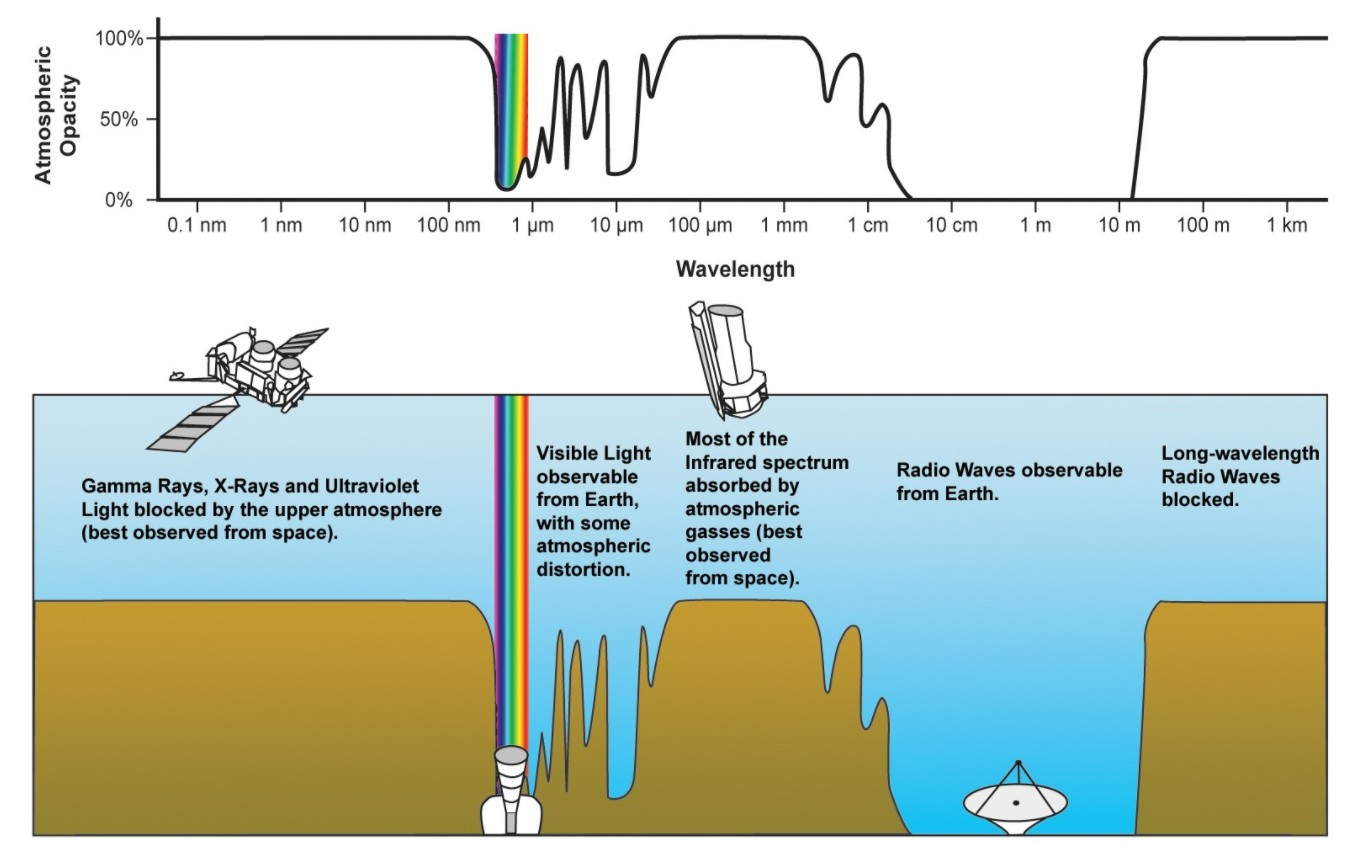
\includegraphics[width=0.8\textwidth]{figures/6-58.jpg}
    
    \caption{Atmospheric absorption percentages throughout the electromagnetic spectrum. Image courtesy of NASA.}
    \label{fig:communication2}
\end{figure}

\textbf{Bruit}

Le bruit est tout signal qui ne fait pas partie de l'information transmise. Il peut s'introduire dans le bilan de liaison à partir du signal d'origine, du système ou de l'environnement.

\begin{figure}[H] % H force l'affichage ici
    \centering
    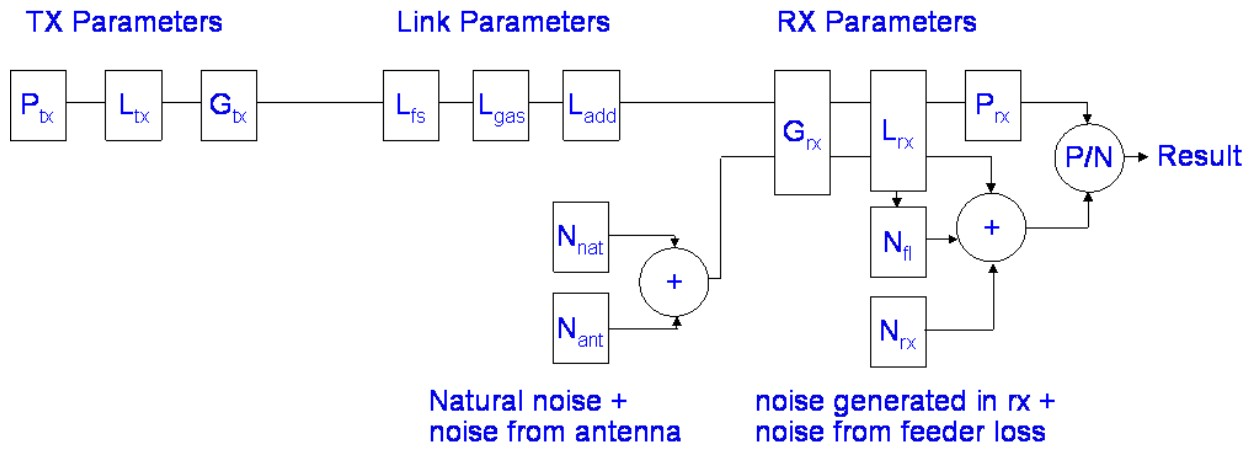
\includegraphics[width=0.8\textwidth]{figures/6-59.jpg}
    
    \caption{Link budgets usually start with the transmitter power and sum all the gains and losses in the system accounting for the propagation losses to find the received power. Then the noise level at the receiver is estimated so we can take the ratio of the signal power to the noise power and work out the performance of the link. Image by Mike Willis.}
    \label{fig:communication2}
\end{figure}

\textbf{• Signal de Bruit}

Le bruit du signal peut se présenter sous la forme de bruit d'amplitude – une erreur dans la magnitude d'un signal – et de bruit de phase – une erreur dans la modulation de fréquence/phase. Le système de communication reçoit ce signal de la charge utile et de divers autres sous-systèmes, nous ne nous attarderons donc pas sur ce point.
\begin{figure}[H] % H force l'affichage ici
    \centering
    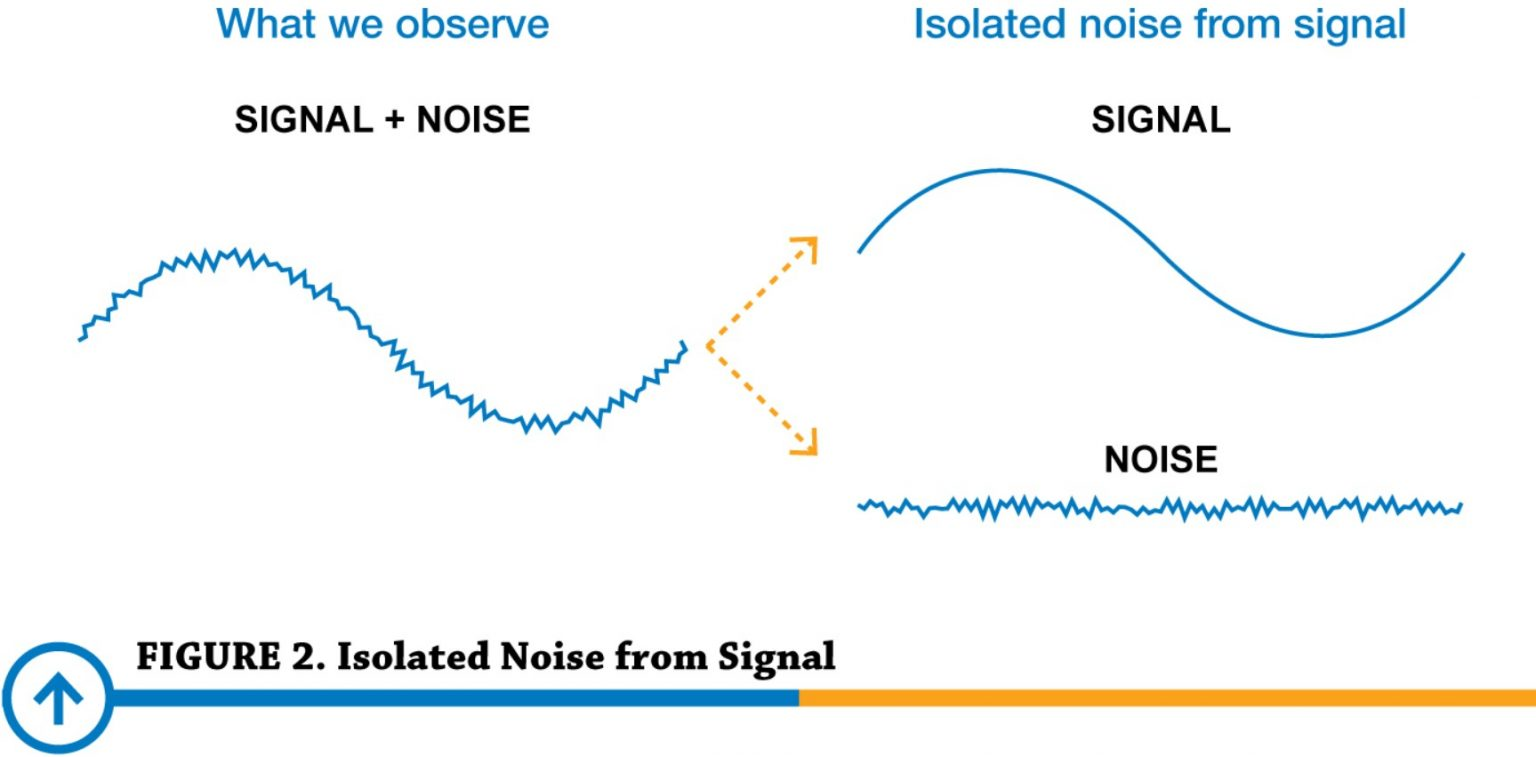
\includegraphics[width=0.8\textwidth]{figures/6-60.jpg}
    
    \caption{Signal noise injected into electrical communication will add or detract from the expected signal value. Image by Predig.}
    \label{fig:communication2}
\end{figure}

\textbf{• Bruit du Système}

Le système de communication présente du bruit dans ses composants sous forme de bruit passif et de bruit actif (amplificateurs, mélangeurs, etc.). Tous les composants réels génèrent un \textit{bruit thermique} dû au mouvement aléatoire des atomes. Le bruit thermique des dispositifs passifs est directement lié à la température du dispositif, à sa bande passante et à la fréquence de fonctionnement. Ce bruit est généré par la vibration thermique des charges liées. Une charge en mouvement génère un signal électromagnétique. Les composants passifs incluent les charges résistives (charges de puissance), les câbles et autres éléments similaires (comme les guides d'ondes). Le bruit total au niveau du récepteur (\(T_s\)) comprend les contributions de l’antenne et du récepteur :

\begin{equation}
    T_s = T_A + T_0(F - 1), \quad T_0 = 290K
\end{equation}

Si la ligne entre l'antenne et le récepteur présente des pertes \(L < 1\), elle contribuera également au bruit :

\begin{equation}
    T_s = T_A + \frac{T_0(F - 1)}{L} + \frac{T_0 (1 - L)}{L}
\end{equation}

où \(T_A\) est la température de bruit de l'antenne, qui dépend de la fréquence et de la direction de pointage de l'antenne, et \(F\) est le facteur de bruit du récepteur. En général, il est possible de réduire le bruit des récepteurs des antennes au sol.

La température de bruit fournit un moyen de déterminer la quantité de bruit thermique générée dans le système de réception. La température de bruit physique d'un dispositif \(T_n\) entraîne une puissance de bruit de :

\begin{equation}
    P_n = K T_n B
\end{equation}

où :

\begin{itemize}
    \item \(K\) : constante de Boltzmann \(K = 1.38 \times 10^{-23} \) J/K ; en dBW, \(K = -228.6\) dBW/K
    \item \(T_n\) : température de bruit de la source en Kelvin
    \item \(B\) : bande passante du dispositif de mesure de puissance en hertz
\end{itemize}

Les systèmes de communication par satellite fonctionnent avec des signaux faibles, il est donc crucial de minimiser le bruit du récepteur autant que possible. En général, la bande passante du récepteur est juste assez large pour laisser passer le signal. Les méthodes permettant de maintenir une faible température du récepteur incluent l'utilisation d'hélium liquide ou d'autres solutions thermiques.

\begin{figure}[H] % H force l'affichage ici
    \centering
    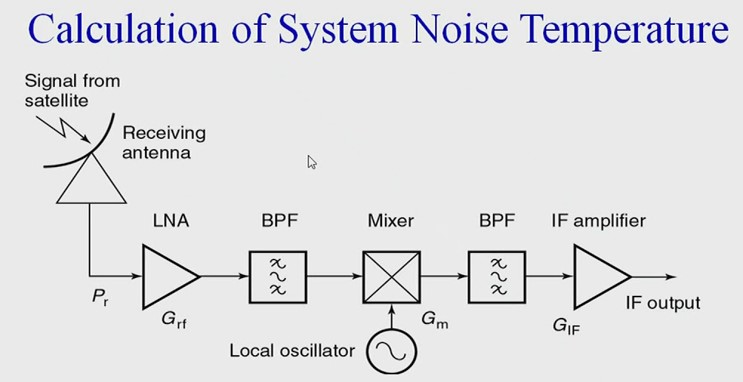
\includegraphics[width=0.8\textwidth]{figures/6-122.jpg}
    
    \caption{An example of system noise temperature. Image by Pravin Yalappa Kumbhar.}
    \label{fig:communication2}
\end{figure}

\textbf{Bruit Environnemental}
Le bruit provenant de l’environnement spatial peut affecter le signal transmis. Il peut être causé par la galaxie, le soleil, l’atmosphère, les précipitations et des sources artificielles.

\textbf{Bruit cosmique} 
Il provient des étoiles présentes dans l’espace. Les étoiles lointaines sont des corps à très haute température, similaires au soleil, et génèrent un bruit comparable. Ce type de bruit est également appelé bruit de corps noir. En plus des étoiles, les galaxies et d’autres sources ponctuelles comme les quasars et les pulsars contribuent également au bruit cosmique.

\begin{figure}[H] % H force l'affichage ici
    \centering
    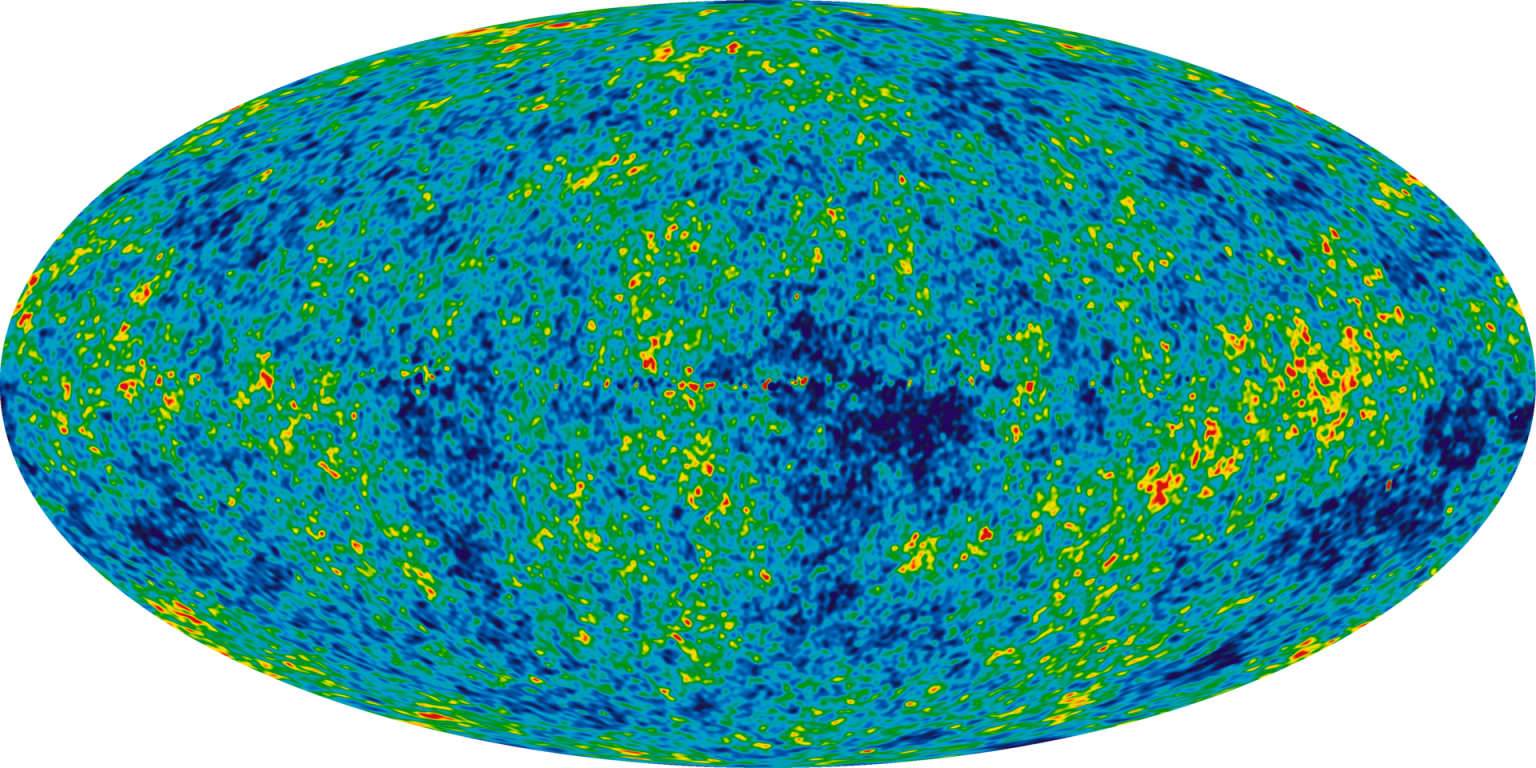
\includegraphics[width=0.8\textwidth]{figures/6-62.png}
    
    \caption{Les fluctuations de température du fond cosmique micro-ondes, mesurées par la sonde Wilkinson Microwave Anisotropy Probe sur sept ans, couvrent l’ensemble du ciel. L’image, en projection Mollweide, montre des variations autour d’une température moyenne de 2,725 K. Les zones rouges sont légèrement plus chaudes et les bleues plus froides d’environ 0,0002 degré. La carte ILC tente d’éliminer le bruit galactique, mais sa fiabilité est limitée, surtout à petite échelle. D’autres cartes sont généralement utilisées pour des analyses scientifiques plus précises.}
    \label{fig:communication2}
\end{figure}

\textbf{Bruit Solaire}

\begin{itemize}
        \item Le Soleil génère du bruit en raison de sa température extrêmement élevée.
        \item Il émet une énergie électrique élevée sous forme de bruit sur une large gamme de fréquences.
        \item L'intensité du bruit varie avec le temps en suivant un cycle de 11 ans.
        \item De fortes perturbations électriques se produisent après chaque cycle de 11 ans.
        \item Durant les autres années, le niveau de bruit est relativement faible.
        \item Les éruptions solaires et les éjections de masse coronale peuvent perturber les communications satellites.
        \item Ces phénomènes peuvent provoquer des rafales de rayonnement susceptibles d’endommager ou de réinitialiser l’électronique des satellites. \end{itemize}

\begin{figure}[H] % H force l'affichage ici
    \centering
    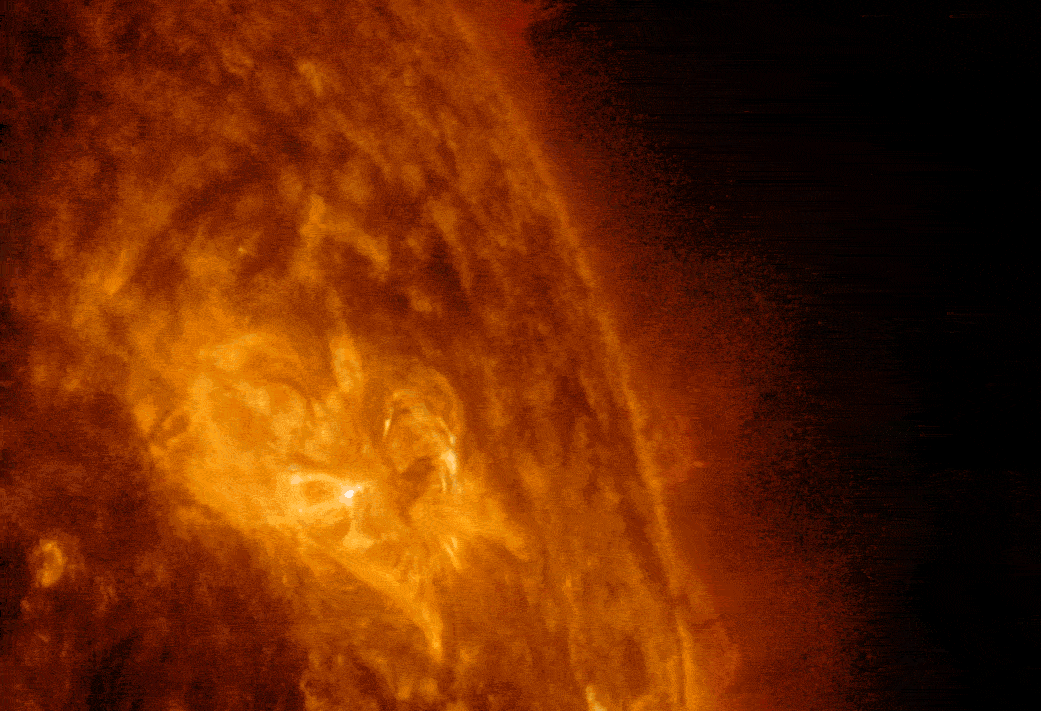
\includegraphics[width=0.8\textwidth]{figures/solar-activity3.en.png}
    
    \caption{NASA’s Solar Dynamics Observatory captured this image of a solar flare, as seen in the bright flash. A loop of solar material, a coronal mass ejection (CME), can also be seen rising up off the right limb of the Sun. Image credit: NASA/SDO/Goddard.}
    \label{fig:communication2}
\end{figure}

\begin{itemize}
    \item \textbf{Effets de l'Atmosphère sur les Communications Satellitaires}
    \begin{itemize}
        \item La pluie entraîne des pertes de signal, en particulier dans la bande Ku.
        \item Les éclairs génèrent des interférences électromagnétiques qui peuvent perturber les communications.
        \item La neige a un impact moindre sur les communications par rapport à la pluie, en raison de sa densité plus faible.
    \end{itemize}
\end{itemize}

\begin{figure}[H] % H force l'affichage ici
    \centering
    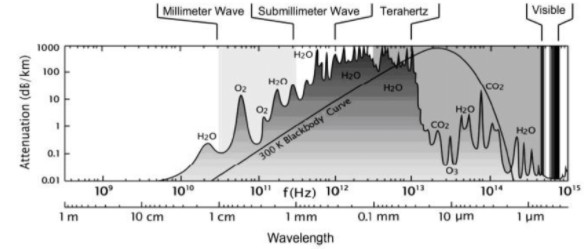
\includegraphics[width=0.8\textwidth]{figures/6-63.jpg}
    
    \caption{Clear atmosphere attenuation of electromagnetic radiation as a function of frequency. Indicated are also the dominant absorption molecules and the Planck law for a 300 K temperature. National Research Council. Assessment of millimeter-wave and terahertz technology for detection and identification of concealed explosives and weapons. National Academies Press, 2007.}
    \label{fig:communication2}
\end{figure}

\textbf{Bruit d'origine humaine}
\begin{itemize}
    \item Les activités humaines génèrent de nombreuses interférences radio qui peuvent perturber les signaux des engins spatiaux.
    \item La Commission fédérale des communications (FCC) régule le spectre radioélectrique pour limiter ces interférences.
    \item Les menaces potentielles pour les communications satellites incluent :
    \begin{itemize}
        \item Les missiles balistiques anti-satellites.
        \item Le brouillage, bien que rare.
    \end{itemize}
\end{itemize}

\begin{figure}[H] % H force l'affichage ici
    \centering
    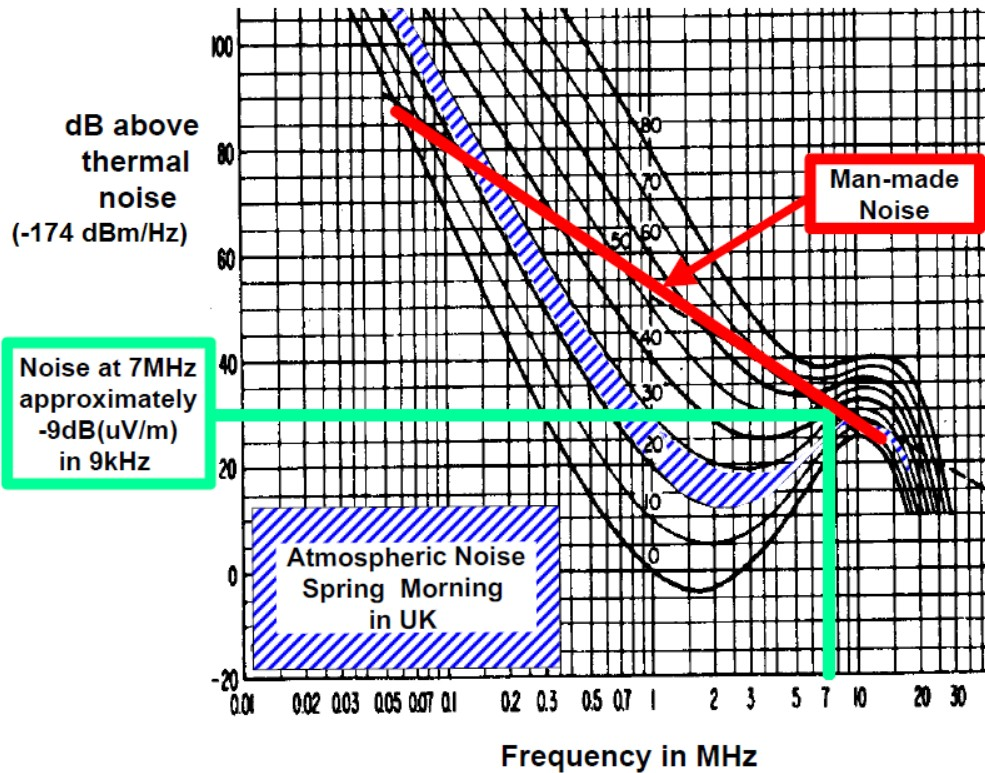
\includegraphics[width=0.8\textwidth]{figures/6-64.jpg}
    
    \caption{Atmospheric noise as a function of frequency in the LF, MF, and HF radio spectrum according to CCIR 322. The vertical axis is in decibels above the thermal noise floor. It can be seen that as the frequency drops atmospheric noise dominates other sources. Image by RSGB.}
    \label{fig:communication2}
\end{figure}

\textbf{Link Margin}

En tant que spécialiste des communications, vous ne devez pas seulement vous assurer que le bilan de liaison est équilibré, mais vous devez concevoir la liaison avec une certaine marge positive par rapport à \(\tfrac{E_b}{N_{0, min}}\) (par exemple, 3 dB).

\begin{equation}
\text{Marge} = \left(\tfrac{E_b}{N_{0}}\right)_{\text{reçu [dB]}} - \left(\tfrac{E_b}{N_{0}}\right)_{\text{requis [dB]}}
\end{equation}

où :

\begin{equation}
\left(\tfrac{E_b}{N_{0}}\right)_{\text{requis [dB]}} = \left(\tfrac{E_b}{N_{0}}\right)_{\text{théorique pour un BER donné}} + \sum \text{Autres pertes système}_{dB}
\end{equation}

En résumé, cette section décrit les différents paramètres qui composent le bilan de liaison et présente des méthodes pour réduire les pertes ou augmenter le gain. Heureusement, de nombreux outils existent pour calculer précisément le bilan de liaison en prenant en compte tous ces paramètres dynamiques. Cependant, il est essentiel d'acquérir une intuition générale pour améliorer le bilan de liaison.

